\documentclass[preprint,12pt]{elsarticle}
% Target journal: Journal of Wind Engineering & Industrial Aerodynamics (Elsevier).
% Format follows the JWEIA guide for authors: numbered references in square brackets (elsarticle-num-names),
% abstract <= 250 words, 1-7 keywords, 3-5 highlights of <= 85 characters (also supplied as highlights.tex),
% graphical abstract (encouraged), declarations of competing interest and of generative AI use, CRediT, data statement.
\usepackage{amsmath,amssymb}
\usepackage{graphicx}
\usepackage[expansion=false]{microtype}
\setlength{\emergencystretch}{1.5em}
\usepackage{booktabs,array}
\usepackage{siunitx}
\usepackage{xcolor}
\usepackage[colorlinks=true,citecolor=blue!60!black,linkcolor=blue!60!black,urlcolor=blue!60!black]{hyperref}
\usepackage{lineno}
\linenumbers
\newcommand{\todo}[1]{\textcolor{red!70!black}{[TODO: #1]}}
\newcommand{\prelim}[1]{\textcolor{orange!80!black}{#1}}   % numbers from a short pilot record, to be replaced
\sisetup{detect-all}
% generated by code/scripts/10_paper_tables.py -- do not edit by hand
\newcommand{\nHours}{287}
\newcommand{\periodStart}{2026-11-13 20:00}
\newcommand{\periodEnd}{2026-11-25 18:00}
\newcommand{\nTrv}{134}
\newcommand{\nSmhi}{17}
\newcommand{\nPairsEighty}{817}
\newcommand{\nSiteHours}{24898}
\newcommand{\ladRawMae}{1.73}
\newcommand{\ladRawBias}{-56}
\newcommand{\ladHeightMae}{1.58}
\newcommand{\ladHeightBias}{-51}
\newcommand{\ladRoughMae}{1.27}
\newcommand{\ladRoughBias}{-44}
\newcommand{\ladSiteMae}{1.27}
\newcommand{\ladSiteBias}{-46}
\newcommand{\ladExpoMae}{0.74}
\newcommand{\ladExpoBias}{-14}
\newcommand{\cvFinalMean}{0.69}
\newcommand{\cvFinalMed}{0.61}
\newcommand{\cvSixMean}{0.72}
\newcommand{\cvSixMed}{0.63}
\newcommand{\cvDiff}{-0.029}
\newcommand{\cvDiffSE}{0.005}
\newcommand{\cvRawMed}{1.47}
\newcommand{\cvRawMean}{2.01}
\newcommand{\cvDir}{17.6}
\newcommand{\cvDirRaw}{19.5}
\newcommand{\cvBetter}{124}
\newcommand{\cvBias}{10}
\newcommand{\cvReduction}{58}
\newcommand{\sfRawMin}{0.40}
\newcommand{\sfRawMax}{2.03}
\newcommand{\sfRawMinName}{Ullared A}
\newcommand{\sfRawMaxName}{Nidingen A}
\newcommand{\sfPotMin}{0.48}
\newcommand{\sfPotMax}{1.82}
\newcommand{\sfPhysShare}{32}
\newcommand{\sfStability}{0.99}
\newcommand{\sfGeoRtwo}{80}
\newcommand{\sfGeoTree}{-0.89}
\newcommand{\sfGeoZo}{-0.074}
\newcommand{\sfGeoCoast}{-0.095}
\newcommand{\sfGeoElev}{0.13}
\newcommand{\coZero}{-0.829}
\newcommand{\coNear}{-0.285}
\newcommand{\coLnxh}{0.092}
\newcommand{\coLnU}{0.223}
\newcommand{\coFar}{-0.123}
\newcommand{\coSmear}{1.18}
\newcommand{\coDzero}{-13.8}
\newcommand{\coDone}{-24.6}
   % numbers produced by code/scripts/15_paper_numbers.py

\journal{Journal of Wind Engineering \& Industrial Aerodynamics}

\begin{document}
\begin{frontmatter}

\title{Correcting weather-station wind to the roadside with open geodata: consequences for estimating the air-drag energy of heavy trucks}

\author[aff1]{\todo{author names, order, ORCID and e-mail of the corresponding author}}
\affiliation[aff1]{organization={\todo{affiliation, or ``Independent researcher''}},
            city={\todo{city}}, country={\todo{country}}}

\begin{abstract}
Wind is a first-order term in the air drag of heavy vehicles, yet the wind a vehicle meets on the road is rarely measured. Synoptic weather stations report wind over open terrain at \SI{10}{m}, whereas roads run close to the ground through forest, valleys and settlements. We quantify and explain how the near-surface wind changes from synoptic stations to roadside road-weather stations, using only open measurements and open geodata, in two regions: Trøndelag--Dovre in Norway (\noTrv{} roadside and \noRef{} reference stations, 2024--2025) and western Sweden (\seTrv{} roadside and \seRef{} reference stations, a \seHours-hour record). The transfer is decomposed into a correction ladder: logarithmic height conversion, two-step roughness conversion through a blending height with roughness lengths from laser-scanned object heights, a persistent site factor for each reference station, and a parsimonious roadside exposure model with trees within \SI{100}{m}, the distance to the forest edge, the regional wind speed and the forest fraction within \SI{1}{km}. Wind estimates from all reference stations are combined with inverse-distance weights. Evaluated out of time and out of station, the median station error of the hourly wind speed falls from \noCvRaw{} to \noCvMed~m\,s$^{-1}$ in Norway and from \seCvRaw{} to \seCvMed~m\,s$^{-1}$ in Sweden, and the median error of the air drag of a tractor--semitrailer at \SI{80}{km.h^{-1}} from \noDragRaw{} to \noDragModel\,\% and from \seDragRaw{} to \seDragModel\,\%. The model form transfers between the countries, but part of the coefficients is regional. At vehicle height, against a van-mounted anemometer on two Norwegian roads, the station-based estimate is more accurate than the nearest stations but less accurate than the MET Nordic analysis, mainly because of direction errors in a mountain valley. The local part of the exposure decorrelates along the road over about \SI{250}{m} in both countries, which bounds the useful length of road segments in vehicle studies.
\end{abstract}


\begin{graphicalabstract}
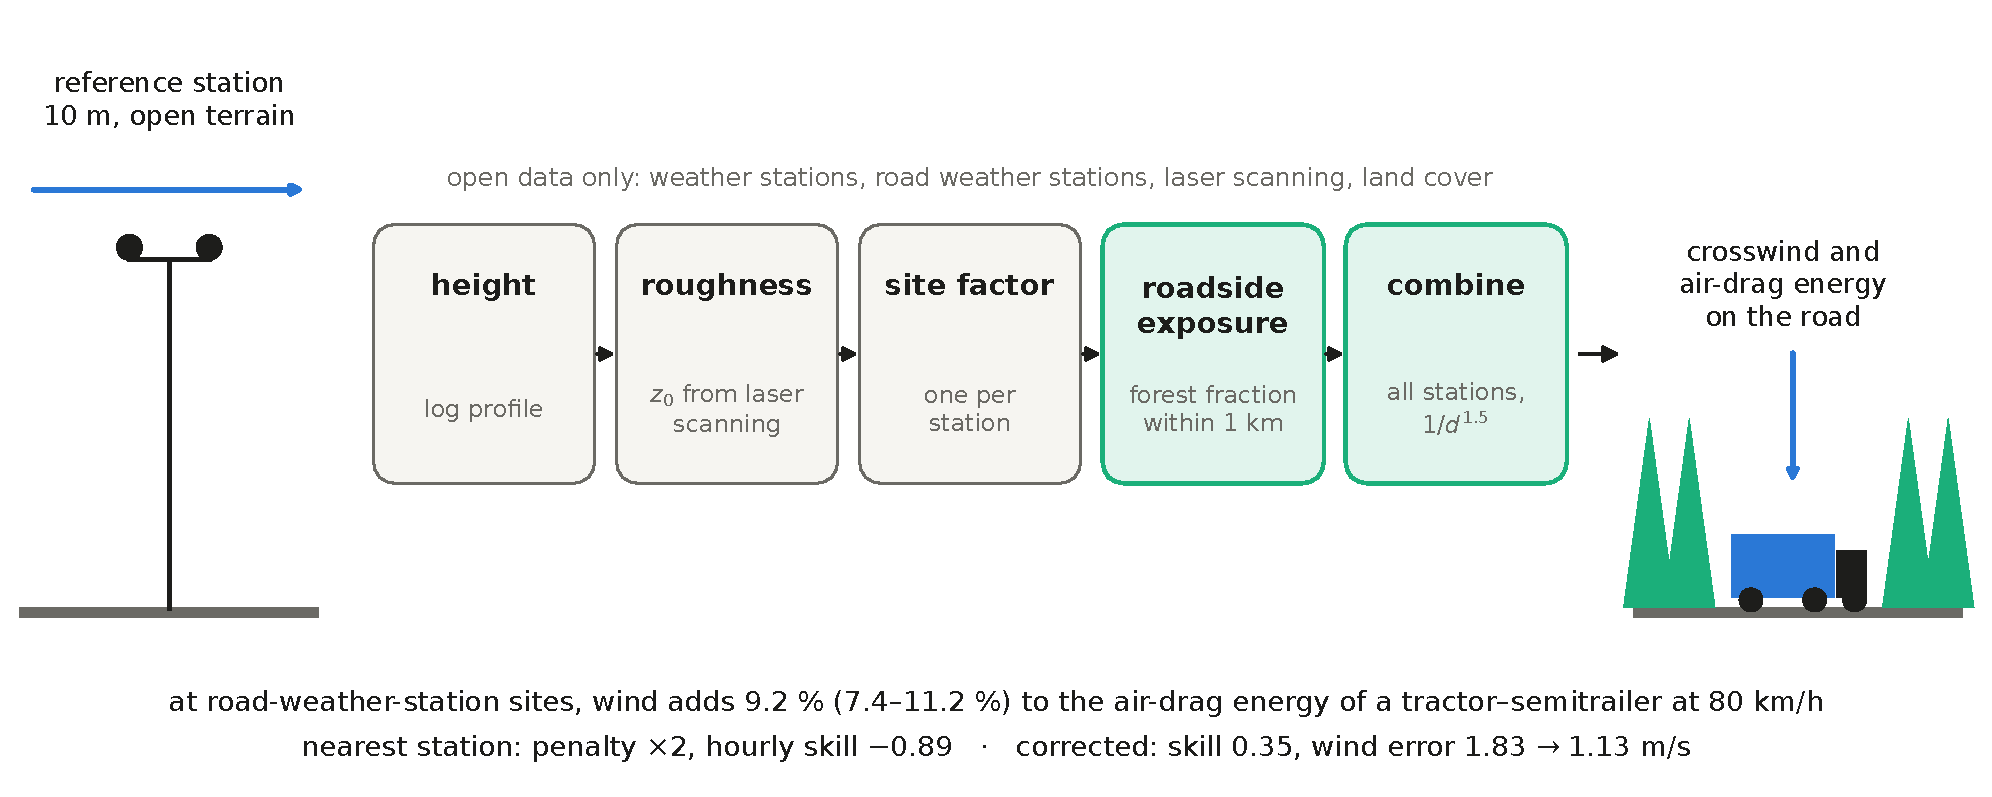
\includegraphics[width=\textwidth]{figures/graphical_abstract.pdf}
\end{graphicalabstract}

\begin{highlights}
\item Station wind is corrected to the roadside with open geodata in Norway and Sweden
\item Forest shelters roads at two scales: trees within 100 m and forest within 1 km
\item Combining all corrected stations is far better than using the nearest station
\item Out-of-sample roadside wind error falls by \noCvRed\,\% in Norway and \seCvRed\,\% in Sweden
\item Exposure decorrelates along roads over $\sim$250 m, bounding vehicle segment length

\end{highlights}

\begin{keyword}
Heavy vehicle air drag \sep Crosswind \sep Energy consumption \sep Road weather station \sep Exposure correction \sep Forest shelter \sep Station-to-site wind transfer
\end{keyword}
\end{frontmatter}

\section*{Nomenclature}
\begin{small}
\begin{tabular}{@{}p{0.15\textwidth}p{0.75\textwidth}@{}}
\multicolumn{2}{@{}l}{\textit{Symbols}}\\
$a(t)$ & network-common term of hour $t$ in the site-factor decomposition\\
$A_f$, $A_s$ & frontal and side area of the vehicle [\si{m^2}]\\
$b_0,\dots,b_4$ & coefficients of the roadside exposure model\\
$C_dA(\beta)$ & drag area at yaw angle $\beta$ [\si{m^2}]\\
$c_s$ & site factor of reference station $s$ (logarithmic)\\
$d_0$, $d_1$ & coefficients of the direction model [\si{\degree}]\\
$d_i$ & distance between a roadside and the $i$-th reference station [km]\\
$F_D$ & air-drag force [N]\\
$F_{1000}$ & fraction of \SI{10}{m} pixels with objects $>\SI{5}{m}$ within \SI{1}{km} (landscape forest fraction)\\
$G_s$, $G_j$ & roughness-conversion factors at the reference and the roadside station\\
$h$ & object height from laser scanning [m]\\
$I$ & turbulence intensity\\
$k(t)$ & 22.5\si{\degree} sector of the wind-from direction of the vector-mean network wind\\
$L$ & e-folding length of the roughness footprint [m]\\
$T_{100}$, $T_{200}$ & fraction of pixels with objects $>\SI{5}{m}$ within 100 or \SI{200}{m} upwind (near-tree share)\\
$U_0,\dots,U_4$ & wind speed after each step of the correction ladder [\si{m.s^{-1}}]\\
$U_j$ & observed roadside wind speed [\si{m.s^{-1}}]\\
$U_\mathrm{net}$ & mean site-corrected wind speed of the reference network [\si{m.s^{-1}}]\\
$v_v$, $v_a$ & vehicle speed and air speed relative to the vehicle [\si{m.s^{-1}}]\\
$v_{wx}$, $v_{wy}$ & head- and crosswind components [\si{m.s^{-1}}]\\
$x/h$ & distance to the first upwind obstacle divided by its height\\
$z_b$ & blending height [m]\\
$z_j$, $z_s$ & sensor height at the roadside and at the reference station [m]\\
$z_0$, $z_{0r}$ & roughness length; reference roughness of open terrain [m]\\
$\alpha$ & angle between the reference wind direction and the road axis\\
$\beta$ & yaw angle of the air flow relative to the vehicle\\
$\rho$ & air density [\si{kg.m^{-3}}]\\
$\varphi$ & wind-from direction\\[3pt]
\multicolumn{2}{@{}l}{\textit{Abbreviations}}\\
MAE & mean absolute error\\
LOSO & leave-one-station-out\\
NWP & numerical weather prediction\\
SE & standard error\\
\end{tabular}
\end{small}

\section{Introduction}
\label{sec:intro}

% Problem
The wind that a truck meets on the road decides a large part of its energy use, yet it is almost never measured. At highway speeds aerodynamic drag is the largest single resistance term of a tractor--semitrailer, and it depends on the air velocity relative to the vehicle: head- and tailwind change the relative speed, and crosswind increases the yaw angle and, through the yaw dependence of the drag area, the drag coefficient \citep{Askerdal2024crosswind}. Over a return trip head- and tailwind partly cancel, crosswind does not. Range prediction for battery-electric trucks therefore needs the local wind along the route \citep{Askerdal2025winter,Shiledar2026}, and strong crosswind is in addition a safety issue for high-sided vehicles \citep{Baker1986,ArayaReyes2026}.

% Why the obvious data source fails
In practice the wind is taken from the nearest weather station or from a numerical weather prediction (NWP) product \citep{Filla2025data,Filla2026}. Both describe the wind at \SI{10}{m} above open, flat terrain, the standard exposure of synoptic observations \citep{WMO8}. A vehicle experiences the wind at \SIrange{2}{4}{m}, often in a corridor cut through forest, along a valley or between buildings. Vehicle measurements make the mismatch concrete. On Canadian highways bordered by forest or terrain, the on-road wind turned with the road and fell to about a fifth of the reference wind when the wind blew across the road \citep{McTavish2024}. In a winter test of a battery-electric truck, the cab-mounted anemometer measured \SI{3.7}{m.s^{-1}} where a station \SI{11}{km} away reported \SI{2.1}{m.s^{-1}} \citep{Askerdal2025winter}. The most complete long-term analysis of truck air resistance from recorded weather therefore lists the unknown height and exposure of the station wind as its main limitation \citep{Filla2026}.

% What others have done (recent)
Two research lines address parts of this problem. Meteorology and wind engineering correct station wind for exposure and roughness \citep{Wieringa1986,Wieringa1993,Verkaik2000}, and recent work has improved the roughness length itself, for example from anemometer towers \citep{Wang2024z0}; large-eddy simulations quantify how forest density, clearings and forest growth change the wind near forests \citep{Chaudhari2026,Topic2026}, and forest growth is a candidate cause of the decline of observed wind in Sweden \citep{Minola2023}. Statistical and deep-learning downscaling map coarse NWP wind to fine terrain \citep{HowardClark2007,Winstral2017,DujardinLehning2022,Dupuy2023,LeToumelin2023,LeToumelin2024,Lian2024}. These studies target wind at \SI{10}{m} or above, in mountains or over open land, evaluated at meteorological stations; a recent study reports that the speed correction learned in the Alps did not transfer to other mountain ranges \citep{LeToumelin2024}. On the vehicle side, on-road and on-bridge measurements characterise channelling and crosswind loads \citep{McTavish2024,Reymert2024,Reymert2025}, yaw-angle distributions have been linked to meteorological data \citep{Xiao2023}, and simplified drag models turn wind into force \citep{Askerdal2024crosswind}. None of these studies quantifies, out of sample and across regions, how station wind must be corrected to represent the wind at the side of a road, nor how much this matters for vehicle drag (Section~\ref{sec:related}).

% Opportunity
Road weather networks offer the missing intermediate reference. The Norwegian Public Roads Administration (Statens vegvesen) and the Swedish Transport Administration (Trafikverket) operate hundreds of roadside anemometers, exposed to the same corridors that vehicles drive through. They do not represent the wind at vehicle height along a whole road, but they are numerous, located on many different roads, and report continuously.

% This study
Here we ask what the wind costs a heavy truck on a given road, and how well this cost can be estimated from open data. We use \noTrv{} Norwegian roadside stations over two years, \noRef{} reference stations and open laser-scanning geodata, with a check in a second landscape in western Sweden, to answer three questions. How much, and why, does the wind change from a synoptic station to the roadside? Can a simple, physically interpretable correction remove most of this change for roads where it was not fitted? And what do the station wind and the corrected wind imply for the air-drag energy of a tractor--semitrailer? We show that stations overestimate the mean roadside wind by \noLadRawBiasAbs\,\%, that the difference is explained by the exposure of each station and by forest at two distinct scales, and that a correction combining all stations reduces the hourly wind error by \noCvRed\,\% out of sample. For the truck, the roadside wind adds on average \enAddNo\,\% to the air-drag energy, almost entirely through crosswind, but the penalty ranges from \enRoadMinNo{} to \enRoadMaxNo\,\% between roads. The nearest-station wind doubles the penalty and predicts the hourly energy worse than ignoring the wind, whereas the corrected wind reproduces the penalty of each road. Its main remaining weakness, the wind direction in mountain terrain, defines the next step.

% Outline
Section~\ref{sec:related} positions the study in recent literature, Section~\ref{sec:data} describes the regions and the data, Section~\ref{sec:methods} the correction chain and the validation design, Section~\ref{sec:results} the results, and Section~\ref{sec:discussion} discusses mechanisms, limits and the use for vehicles.

\section{Related work and contribution}
\label{sec:related}

We reviewed twenty studies from 2023--2026 found by keyword searches on wind downscaling, station exposure and roughness, forest flow, on-road wind measurement and the effect of wind on vehicle energy, together with the classical references they build on. Table~\ref{tab:literature} summarises the most relevant ones by what they predict, what they use as truth, how they validate and whether they reach the vehicle.

\begin{table}[!htbp]
\centering
\caption{Representative studies on the wind near roads and vehicles. Height: height of the predicted wind. Truth: observations against which the method is evaluated. Held out: whether evaluation sites (S) or periods (T) were withheld, or another region (R); --: not done or not reported.}
\label{tab:literature}
\footnotesize
\setlength{\tabcolsep}{3pt}
\begin{tabular}{>{\raggedright\arraybackslash}p{0.16\textwidth}>{\raggedright\arraybackslash}p{0.14\textwidth}>{\raggedright\arraybackslash}p{0.2\textwidth}>{\raggedright\arraybackslash}p{0.2\textwidth}>{\centering\arraybackslash}p{0.07\textwidth}>{\raggedright\arraybackslash}p{0.11\textwidth}}
\toprule
Study & Height, setting & Truth & Method & Held out & Vehicle link \\
\midrule
\citet{DujardinLehning2022} & 10\,m, Alps & meteorological stations & CNN, NWP + terrain & S & -- \\
\citet{Dupuy2023} & 10\,m, SE France & 1\,km WRF fields & CNN, 9\,km $\to$ 1\,km & -- & -- \\
\citet{LeToumelin2024} & 10\,m, Alps & 273 stations & NN correction + CNN downscaling & S, T, R & -- \\
\citet{Lian2024} & near-surface, E China & stations & deep learning, terrain + station links & -- & -- \\
\citet{TroenPetersen1989} & 10--100\,m, wind resource & masts & roughness, obstacle and orography models (WAsP) & S & -- \\
\citet{Herb2007} & along railway tracks & stations & standards-based roughness and orography transfer & -- & rail crosswind risk \\
\citet{Wang2024z0} & roughness length & 101 towers & $z_0$ from tower profiles & -- & -- \\
\citet{Chaudhari2026}; \citet{Topic2026} & canopy to hub height & tower data & LES with forest from laser scanning & -- & -- \\
\citet{McTavish2024} & 1--3\,m on road, Canada & vehicle probes & measurement, video classification & -- & chan\-nel\-ling \\
\citet{Reymert2024,Reymert2025} & vehicle, Norwegian bridges & vehicle anemometer, GNSS/IMU & Kalman filter for crosswind loads & -- & cross\-wind load \\
\citet{Filla2025data,Filla2026} & 6\,m station = vehicle & none for wind & nearest road weather station & -- & drag, 5 years \\
\citet{Askerdal2024crosswind,Askerdal2025winter} & vehicle & CFD; truck anemometer & simplified $C_dA(\beta)$; motion resistance & -- & drag \\
\textbf{This study} & roadside (10\,m) and vehicle (3.4\,m) & \noTrv{} roadside stations (\seTrv{} for development); van anemometer & physical ladder + parsimonious exposure model, four baselines & S, T & drag energy \\
\bottomrule
\end{tabular}
\end{table}

Three gaps stand out. First, downscaling studies predict the wind at \SI{10}{m} over terrain and are evaluated at meteorological stations, which are sited to avoid the sheltered places where roads run; the roadside wind is not their target. Their skill can also be regional: the speed correction of \citet{LeToumelin2024} degraded outside the Alps. Second, roughness and forest studies explain the physics but do not provide a correction that can be evaluated against an independent network. Third, vehicle studies either measure the on-road wind on a few routes \citep{McTavish2024,Reymert2024} or use station wind without correction \citep{Filla2026}, so that the error of the station wind at the road is unknown.

This paper contributes to closing these gaps in four ways. (i) It uses a national road weather network as the truth for the station-to-roadside transfer, with blocked-time $\times$ leave-one-station-out validation over 23 months and a hold-out year, and compares the correction with the alternatives that a practitioner would use: the nearest station rescaled by one constant, the nearest other road weather station, and a 1-km NWP analysis, raw, rescaled by one constant and combined with the exposure model. (ii) It decomposes the transfer into physically interpretable steps using open laser-scanning data and shows which of them matter. (iii) It quantifies the wind penalty in the air-drag energy of a tractor--semitrailer at the station sites, with its uncertainty, and shows how the choice of wind source biases it. (iv) It tests the result at vehicle height and reports where the correction fails, including strong wind and wind direction.

\section{Study region and data}
\label{sec:data}

\subsection{Region}
The study region is Trøndelag--Dovre in central Norway, within \SI{170}{km} of \ang{63.2}\,N, \ang{10.0}\,E (Fig.~\ref{fig:map-no}). It spans the outer coast with islands and skerries, the Trondheimsfjord, forested valleys and the Dovre mountain plateau above \SI{1000}{m}; the roads follow valleys and fjords, so that the region contains open coastal roads, forest corridors, valley roads and mountain passes within a few hours' drive. This variety of road environments is the reason for choosing it.

\begin{figure}[!htbp]
\centering
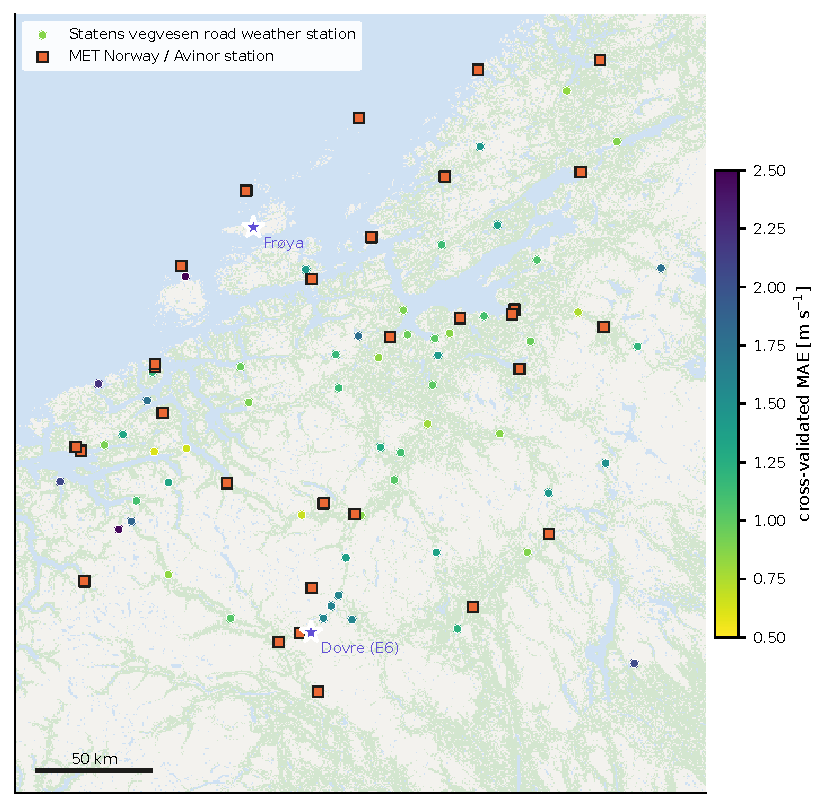
\includegraphics[width=\textwidth]{figures/fig01_norway_area.pdf}
\caption{Study region: reference stations of MET Norway and Avinor (squares), road weather stations of Statens vegvesen (circles, coloured by the cross-validated mean absolute error of the corrected hourly wind speed) and the two road sections with vehicle measurements (stars). Background: forest, open land and water from ESA WorldCover.}
\label{fig:map-no}
\end{figure}

\subsection{Reference stations}
The reference network consists of the \noRef{} stations of MET Norway and Avinor (airports) in the region that report hourly wind at \SI{10}{m}, obtained from the Frost API of MET Norway \citep{Frost}. The year 2023 was used only to estimate the site factors of the reference stations (Section~\ref{sec:methods}).

\subsection{Roadside stations}
Statens vegvesen road weather stations report 10-min wind, distributed through Frost with a nominal sensor level of \SI{10}{m} above ground; on-the-hour values from \noStart{} to \noEnd{} (\noHours{} hours) were used. Speeds were checked for implausible values ($>\SI{60}{m.s^{-1}}$) and stuck sensors (the same non-zero value in six or more consecutive hours, or zero in twelve or more), which removed \noQcPct\,\% of the values; the \noTrv{} stations with at least 2000 valid hours were retained.

\subsection{Geodata}
Object heights were taken from airborne laser scanning, as the difference between the national digital surface and terrain models of Kartverket \citep{Kartverket}, resampled to \SI{10}{m}; objects higher than \SI{5}{m} are counted as trees or obstacles. Open water was taken from ESA WorldCover \citep{WorldCover}. The road axis at each roadside station was obtained by snapping the station to the OpenStreetMap road network with OSRM \citep{Luxen2011}.

\subsection{Vehicle measurements}
The NOR-XWIND data set \citep{NORXWIND} contains wind measured with an ultrasonic anemometer on a van (sensor \SI{3.4}{m} above ground) together with high-rate GNSS and inertial data \citep{Reymert2025}. Two road sections lie in the region: the E6 across the Dovre mountains (2020-10-29 and 2020-10-31) and the open coast of Frøya (2020-11-05). The anemometer orientation and gain were calibrated with the consistency of opposite driving directions, and the ground-fixed wind was averaged over road segments. There are \vehN{} segment passages (\vehNDovre{} at Dovre, \vehNFroya{} at Frøya), but they fall in only \vehHours{} distinct hours (\vehHoursDovre{} and \vehHoursFroya{}), so that the vehicle validation is a case study rather than a statistical test. The MET Nordic analysis \citep{MetNordic,Nipen2020}, a post-processed product of the MetCoOp ensemble prediction system \citep{Muller2017}, was interpolated to the segments and is used as an independent benchmark.

\subsection{Independent check region}
To test whether the findings hold in a different landscape, the same analysis was repeated in a flat-to-hilly, forest-dominated region within \SI{120}{km} of road RV40 between Gothenburg and Borås in western Sweden, with \seRef{} synoptic stations of SMHI \citep{SMHIopen} and \seTrv{} Trafikverket road weather stations at \SI{6}{m} \citep{TRVapi}. Because the Trafikverket API keeps only seven days, this record covers \seHours{} hours in November 2026. Object heights came from the NMD layer of Naturvårdsverket \citep{NMD}. Details are given in \ref{app:sweden}; the main text reports the Swedish results only where they confirm or contradict the Norwegian ones.

\section{Methods}
\label{sec:methods}

\subsection{Overview}
Figure~\ref{fig:concept} illustrates the idea. The wind measured at a reference station is first converted to the wind at the height of the roadside sensor over open terrain, then corrected for the roughness around both sites and for the persistent exposure of the reference station, and finally for the shelter of the road corridor; the estimates of all reference stations are then combined. For a roadside station $j$ and a reference station $s$ the hourly wind speed is transferred in four steps,
\begin{equation}
U_0 \xrightarrow{\text{height}} U_1 \xrightarrow{\text{roughness}} U_2 \xrightarrow{\text{site factor}} U_3 \xrightarrow{\text{roadside exposure}} U_4 ,
\label{eq:ladder}
\end{equation}
and the estimates from all reference stations are combined (Section~\ref{sec:combine}). Direction-dependent quantities are evaluated in the 16 sectors of the wind-from direction of the vector-mean wind of the reference network, $k(t)$. Each step is evaluated separately, so that its contribution to the error reduction can be read directly. The same model, with the same predictors, is fitted separately in each country.

\begin{figure}[!htbp]
\centering
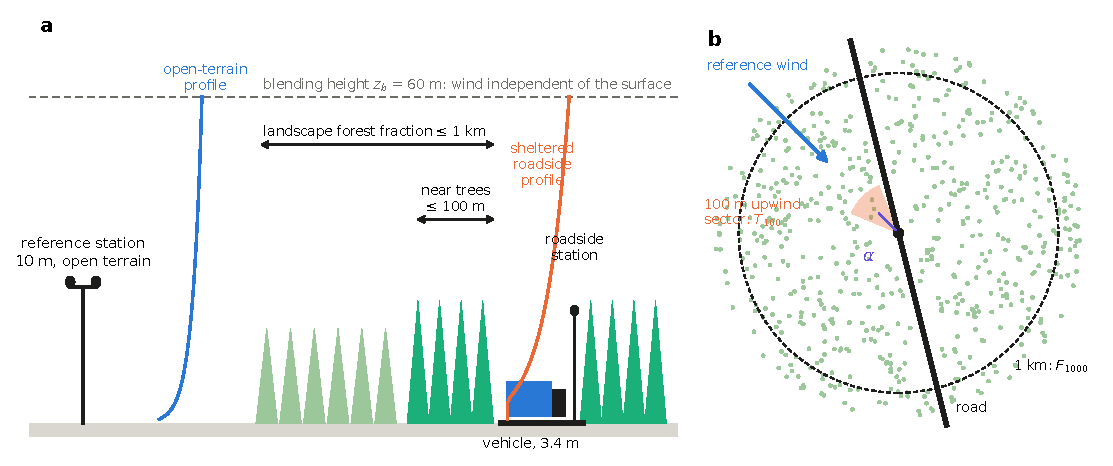
\includegraphics[width=\textwidth]{figures/fig00_concept.pdf}
\caption{The problem and the predictors. (a) Side view: the reference station measures over open terrain at \SI{10}{m}; above the blending height the wind is independent of the surface; at the road, trees next to the road and the forest of the surrounding landscape reduce the wind at the roadside sensor and at the vehicle. (b) Plan view of the exposure predictors at a roadside station: the near-tree share $T_{100}$ in the upwind sector within \SI{100}{m}, the forest fraction $F_{1000}$ within \SI{1}{km} in all directions, and the angle $\alpha$ between the reference wind and the road axis, which controls the deflection of the wind direction. Schematic, not to scale.}
\label{fig:concept}
\end{figure}

\subsection{Height conversion}
Under neutral stratification over open terrain ($z_{0r}=\SI{0.03}{m}$),
\begin{equation}
U_1 = U_0\,\frac{\ln(z_j/z_{0r})}{\ln(z_s/z_{0r})},
\end{equation}
with $z_s=\SI{10}{m}$; $z_j=\SI{6}{m}$ in Sweden (factor 0.912) and $\SI{10}{m}$ in Norway (factor 1). The same open-terrain profile converts every wind to vehicle height, $z=\SI{3.4}{m}$ (factor 0.814 from \SI{10}{m}); Section~\ref{sec:energy-method} gives the sensitivity of the results to this choice.

\subsection{Roughness conversion}
Following \citet{Wieringa1986}, the wind at a blending height $z_b=\SI{60}{m}$ is assumed to be independent of the local surface. The measured wind is converted to the potential wind over open terrain and then to the roadside,
\begin{align}
G_s(z_0) &= \frac{\ln(z_b/z_0)}{\ln(z_s/z_0)}\,\frac{\ln(z_s/z_{0r})}{\ln(z_b/z_{0r})}, \qquad
G_j(z_0) = \frac{\ln(z_b/z_{0r})}{\ln(z_s/z_{0r})}\,\frac{\ln(z_j/z_0)}{\ln(z_b/z_0)},\\
U_2 &= U_0\,G_s\!\left(z_{0,s}(k)\right)\,G_j\!\left(z_{0,j}(k)\right).
\end{align}
The effective roughness length in sector $k$ is a footprint-weighted geometric mean over the \SI{10}{m} pixels within $\pm\ang{22.5}$ of the upwind direction, with weights $e^{-r/L}$, $L=\SI{100}{m}$, and $z_{0}=0.1\,h$ where the object height $h>\SI{5}{m}$, \SI{0.0002}{m} over water and $z_{0r}$ elsewhere. No zero-plane displacement is used: the roadside sensors stand in clearings and corridors, below or at the height of nearby canopies, where the logarithmic profile does not strictly hold \citep{Raupach1994,Finnigan2000}; the conversion is therefore a first-order correction whose residual is left to the empirical exposure model.

\subsection{Site factors of the reference stations}
Each reference station has a persistent exposure that the roughness conversion captures only partly (coast, hill tops, valleys, nearby obstacles). On the training period the potential wind is decomposed as
\begin{equation}
\ln U_{\mathrm{pot},s}(t) = a(t) + c_s + \varepsilon_{s}(t),\qquad \sum_s c_s=0,
\end{equation}
where $a(t)$ is the network-common term of hour $t$ and $c_s$ the site factor of station $s$, fitted by alternating least squares on hours with a network median speed $\ge\SI{3}{m.s^{-1}}$ and at least 12 reporting stations. The corrected wind is $U_3 = U_2\,e^{-c_s}$. Direction-dependent site factors were tested and did not improve the result (Section~\ref{sec:res-sens}).

\subsection{Roadside exposure model}
The remaining ratio between the roadside observation and $U_3$ is modelled as
\begin{equation}
\ln\frac{U_j}{U_3} = b_0 + b_1\,T_{100}(k) + b_2 \ln\frac{x}{h}(k) + b_3 \ln U_{\mathrm{net}} + b_4\,F_{1000} + \varepsilon ,
\label{eq:exposure}
\end{equation}
where $T_{100}$ is the fraction of pixels with objects $>\SI{5}{m}$ within \SI{100}{m} upwind ($\pm\ang{22.5}$), $F_{1000}$ the same fraction within \SI{1}{km} in all directions (the forest fraction of the landscape), $x/h$ the distance to the first upwind obstacle divided by its height (median over seven rays in the sector, capped at \SI{1500}{m}) and $U_{\mathrm{net}}$ the mean site-corrected wind of the reference network. The model is fitted by ordinary least squares on station pairs and hours with $U_0\ge\SI{2}{m.s^{-1}}$, a roadside speed above \SI{0.2}{m.s^{-1}} and all predictors available; the back-transformation uses the smearing estimate \citep{Duan1983}, computed without the predicted roadside station. The form of Eq.~\eqref{eq:exposure} results from the selection described in Section~\ref{sec:validation}.

\subsection{Wind direction}
Road corridors deflect the wind towards the road axis. With $\alpha$ the angle between the reference wind direction and the road axis,
\begin{equation}
\varphi_j = \varphi_s + d_0 + d_1 \sin(2\alpha)\,T_{200},
\end{equation}
a form analogous to the terrain-diverting factor of \citet{ListonElder2006}, fitted by least squares on the wrapped direction difference in hours with $U_0\ge\SI{3}{m.s^{-1}}$ and a roadside speed of at least \SI{1.5}{m.s^{-1}}.

\subsection{Combination of the reference stations}
\label{sec:combine}
The roadside wind speed is the weighted geometric mean of the estimates $U_{4,i}$ from all reference stations within \SI{150}{km} (\SI{120}{km} in Norway), with weights $w_i = d_i^{-1.5}$ ($d_i$ distance, floored at \SI{3}{km}); the direction is the weighted vector mean from stations within \SI{60}{km} ($w_i=d_i^{-1}$; the nearest station if none is within \SI{60}{km}).

\subsection{Comparison estimators}
\label{sec:baselines}
The corrected estimate is compared with four alternatives that need no exposure model. \emph{Nearest station}: the nearest reference station with data in the hour, converted to the sensor height. \emph{Rescaled nearest station}: the same multiplied by one constant, the ratio of the mean roadside to the mean nearest-station wind, learned on the other time blocks and the other roadside stations. \emph{Nearest road station}: the wind of the nearest other road weather station with speed and direction in the hour; this is what a practitioner with access to the road weather network would use. \emph{MET Nordic}: the analysis interpolated to the station (Section~\ref{sec:data}). All estimators are scored on the same hours. Because the exposure model is fitted in log space, its estimate can be conditionally biased; a recalibrated variant multiplies it by the ratio of the mean observed to the mean estimated wind in bins of the estimate, again learned on the other blocks and stations.

\subsection{Validation design}
\label{sec:validation}
Parameters are never evaluated on the data used to fit them. The test period is divided into consecutive time blocks---eight blocks of about three months in Norway, so that every season is left out once, and four blocks of about three days in Sweden. The exposure and direction models are fitted on all blocks but one and on all roadside stations except the one predicted (leave-one-station-out, LOSO), and evaluated on the remaining block; every prediction is therefore out of time and out of station \citep{Roberts2017}. Site factors are estimated only from the year before the test period. The score is the mean absolute error (MAE) of the hourly wind speed per roadside station, summarised by the median over stations; two settings are compared with paired differences per station and their standard error (SE). The bias is reported as the ratio of the mean estimated to the mean observed wind speed minus one, over all hours with both values. Uncertainty across stations is given as 95\,\% intervals from a station-cluster bootstrap (2000 resamples of stations); it is the relevant uncertainty because the exposure predictors vary only between stations and sectors.

The predictors and the form of the station combination were chosen on the Swedish record (\ref{app:sweden}) and then fitted anew in Norway. Length scales and thresholds were varied one at a time; a value is retained when it is within one standard error of the best value of its group \citep{Hastie2009}, preferring the physically better founded or simpler one. Because these choices were scored with the same cross-validation that is reported, all Norwegian choices were also repeated on 2024 alone (four blocks), and the resulting model, fitted on 2024, was evaluated leave-one-station-out on the untouched year 2025. Terrain indices from the Norwegian terrain model---the upwind shelter index $S_x$ \citep{Winstral2002} within \SI{300}{m} and \SI{1}{km}, the topographic position index within \SI{500}{m} and \SI{2}{km}, and the relief within \SI{2}{km}---were tested as additional predictors of the final model.

\subsection{Transfer between the countries}
To test whether the fitted model can be used in a region without roadside stations, the coefficients of Eq.~\eqref{eq:exposure} and of the direction model fitted in one country are applied unchanged in the other; the physical steps and the site factors use the local data.

\subsection{Application at vehicle height}
For the NOR-XWIND segments, the model fitted on all Norwegian roadside data is applied with the segment's own features and the reference observations of the hour nearest to the passage. It predicts the wind that a \SI{10}{m} roadside anemometer at the segment would measure; this is converted to \SI{3.4}{m} with the same open-terrain factor as all other estimates (sensitivity: the local-$z_0$ profile). It is compared with no wind, the nearest reference station and the nearest road weather station, both converted in the same way, and with the MET Nordic analysis at \SI{10}{m}, converted in the same way. Because the station-based estimates are hourly, results are averaged per reference hour, and intervals are obtained by resampling hours.

\subsection{Air drag and energy}
\label{sec:energy-method}
Wind is propagated to the air drag of a tractor--semitrailer with
\begin{align}
F_D &= \tfrac12 \rho\, C_dA(\beta)\, v_a^2, & v_a^2 &= (v_v+v_{wx})^2+v_{wy}^2, & \beta &= \arctan\frac{|v_{wy}|}{v_v+v_{wx}},
\label{eq:drag}
\end{align}
with the vehicle speed $v_v$, the head- and crosswind components $v_{wx}$ (positive against the direction of travel) and $v_{wy}$, the air speed $v_a$, the yaw angle $\beta$ and $\rho=\SI{1.25}{kg.m^{-3}}$. The drag area at zero yaw is $C_dA(0)=\SI{5.8}{m^2}$, the typical value certified for EU 4$\times$2 long-haul tractor--trailers \citep{ICCT_VECTO}. Its yaw dependence follows the generic speed-dependent crosswind correction for tractor--semitrailers of VECTO, the simulation tool of the EU certification of heavy-duty vehicles \citep{EU2017_2400,VECTO},
\begin{equation}
C_dA(\beta) = C_dA(0) + a_1\beta + a_2\beta^2 + a_3\beta^3,
\label{eq:vecto}
\end{equation}
with $a_1=0.030042$, $a_2=0.040817$, $a_3=-0.002130$, $\beta$ in degrees and $C_dA$ in \si{m^2}, held constant beyond its maximum at $\beta=\ang{13.1}$ (a 45\,\% increase), which is exceeded in \enCapPctNo\,\% of the passes. As an upper bound of the crosswind sensitivity we also use Model~1 of \citet{Askerdal2024crosswind}, $C_dA(\beta)\propto\cos^2\beta\,(A_f\cos\beta+A_s\sin\beta)$ with $A_f=\SI{10.3}{m^2}$ and $A_s=\SI{57.6}{m^2}$, scaled to the same $C_dA(0)$; it nearly doubles the drag area at \ang{10} yaw, where Eq.~\eqref{eq:vecto} gives \SI{39}{\percent}.

The energy needed to overcome air drag per distance equals the force; we report it in \si{kWh} per \SI{100}{km} at the wheel. At each roadside station with adequate direction coverage and each hour a vehicle is driven in both directions along the road axis at \SI{80}{km.h^{-1}} (sensitivity: 60--\SI{90}{km.h^{-1}}); a round trip is the mean of both directions. The results therefore describe the station sites, which are not a random sample of the road network. All winds---observed and estimated---are referred to vehicle height (\SI{3.4}{m}) with the same open-terrain factor, so that this conversion does not favour any estimator. We define the wind penalty as the air-drag energy with wind minus that in still air, relative to the still-air energy; it does not depend on the air density, whose range in the region (about 1.15--\SI{1.32}{kg.m^{-3}} between warm lowland and cold mountain conditions) changes the absolute energy by $-8$ to $+6$\,\% relative to the value of \SI{1.25}{kg.m^{-3}} used here. Head/tail-only and crosswind-only penalties are computed with one wind component set to zero; because Eq.~\eqref{eq:drag} is not additive in the components, they do not sum exactly to the total.

The size of the penalty depends on assumptions that cannot be checked with the roadside data. Its uncertainty is explored by repeating the calculation with the observed wind and (i) a sensor height of \SI{6}{m} instead of \SI{10}{m}; (ii) roughness lengths of 0.01--\SI{0.3}{m}, with and without a displacement height of \SI{2}{m}, and no height reduction at all for the profile from \SI{10}{m} to \SI{3.4}{m}; (iii) Model~1 instead of the VECTO curve; and (iv) a turbulence correction, averaging Eq.~\eqref{eq:drag} over Gaussian longitudinal and lateral fluctuations of the wind with standard deviations $\sigma_u=I\,U$ and $\sigma_v=0.8\,\sigma_u$, $I=0.15$ and $0.3$, a simple form of the wind-averaged drag \citep{Windsor2014,WordleySaunders2008}.

The estimators of Section~\ref{sec:baselines}, and no wind (common practice in range prediction), are compared by the mean absolute error of the hourly one-way energy, its skill score $1-\mathrm{MSE}/\mathrm{MSE}_\text{no wind}$, the long-term penalty of each station site (mean over all hours and both directions) and its correlation with the observed penalty, and the error in hours with a substantial wind effect, in which the observed wind changes the air-drag energy by at least \SI{10}{\percent}. Intervals are from the station-cluster bootstrap. For the vehicle segments, the energy is evaluated along the measured heading.

\section{Results}
\label{sec:results}
% All numbers in orange are from the 12-day pilot (2026-11-13 to 11-25) and will be replaced.

\subsection{Raw discrepancy between the networks}
\todo{Table 1: raw ratio TrV/SMHI by station type; Fig.~2: scatter / ratio distribution.} With the nearest SMHI station scaled to \SI{6}{m}, the median station MAE is \prelim{1.5}~m\,s$^{-1}$ and the roadside wind is on average \prelim{about half} of the synoptic wind.

\subsection{Correction ladder}
\todo{Table 2 and Fig.~3: MAE, bias and correlation after each step of Eq.~\eqref{eq:ladder}.} Pilot values (median over 813 station pairs): MAE \prelim{1.75 $\rightarrow$ 1.56 $\rightarrow$ 1.37 $\rightarrow$ 1.30 $\rightarrow$ 0.74}~m\,s$^{-1}$; bias \prelim{$-57\% \rightarrow -14\%$}.

\subsection{Site factors of the synoptic stations}
\todo{Fig.~4: site factors by station and sector; table of geographic regression.} Pilot: factors range from \prelim{$\times0.40$ to $\times2.05$}; split-half stability \prelim{$r=0.99$}; the roughness conversion explains \prelim{about 40\%} of their variance; four geographic predictors explain \prelim{80\%} (leave-one-station-out).

\subsection{Roadside exposure model}
\todo{Table 3: coefficients with time-block ranges; partial-effect plots.} Pilot coefficients: near trees \prelim{$-0.30$}, forest within 1~km \prelim{$-0.16$}, $\ln(x/h)$ \prelim{$+0.09$}, $\ln U_\mathrm{net}$ \prelim{$+0.28$}, $\Delta T$ \prelim{$+0.023$~K$^{-1}$}.

\subsection{Sensitivity to length scales and thresholds}
\todo{Fig.~5: one-at-a-time sensitivity panels; Fig.~6: near $\times$ far tree-scale grid; Table 4: recommended ranges.}

\subsection{Along-road correlation of exposure}
\todo{Fig.~7: correlation of upwind features along the road; effect of segment-averaged features.} Pilot: local part decorrelates over \prelim{about 250~m}.

\subsection{Combination and value of individual synoptic stations}
\todo{Fig.~8: error vs number/radius of stations; station value controlled for distance and roadside station.}

\subsection{Wind direction}
\todo{}

\subsection{Implication for air-drag estimation}
\todo{}

\section{Discussion}
\label{sec:discussion}

\subsection{Why the wind changes from the station to the road}
The results separate three causes of the difference between synoptic and roadside wind. The measurement height and the local roughness explain a large part in a forested lowland such as western Sweden, where synoptic stations stand in open terrain and roads run through forest; the logarithmic wind profile and the blending-height concept \citep{Wieringa1986} capture this with fixed physical constants and are insensitive to their exact values. Second, each reference station has a persistent exposure of its own, of a factor up to two in either direction (\noSfMin--\noSfMax{} in Norway), which must be removed before stations can be combined; a single factor per station suffices. Third, and most important at the roadside, the wind is reduced by forest at two distinct scales: the trees next to the road, within a few tree heights, and the forest fraction of the surrounding landscape within about \SI{1}{km}. The first scale corresponds to the sheltered zone behind forest edges and windbreaks \citep{HeislerDeWalle1988,DupontBrunet2008}; the second to the roughness of the landscape that controls the near-surface wind through the internal boundary layer. The absence of any effect at intermediate radii of \SIrange{300}{500}{m}, found in both countries, supports this two-scale view.

In mountainous Norway the landscape forest fraction dominates, the physical roughness conversion adds little, and explicit terrain indices did not help. A plausible reason is that the forest fraction already acts as a proxy for terrain: in central Norway forest grows in sheltered valleys, while exposed plateaus and coasts are open. The near-tree coefficient changes sign between the countries for the same reason; it should be read together with the forest fraction, not as an independent physical effect.

\subsection{Combining stations}
The single largest improvement comes from combining all reference stations within about \SI{100}{km} rather than taking the nearest one, after the site factors have made them comparable. A single station, even nearby, carries its own exposure and its own local turbulence; averaging many corrected stations recovers the regional wind, which the roadside exposure model then localises. This agrees with the common practice of using the regional flow from an analysis or model rather than a single observation, and explains why the MET Nordic analysis, which combines observations with a numerical model, is a strong benchmark at vehicle height.

\subsection{Transferability}
The model form---the same predictors and the same physical steps---works in both landscapes, and its coefficients are stable in time within each country. The coefficients, however, are partly regional: transferred to the other country, the model keeps a clear advantage over the nearest station in Sweden but only a small one in Norway. For a new region with roadside stations the coefficients should therefore be refitted, which requires only open data; for a region without roadside stations, the coefficients of the most similar landscape should be used and the uncertainty reported. The feature distributions of the training stations define the domain of applicability: mountain passes, bridges and urban street canyons are underrepresented in both data sets.

\subsection{Use for vehicles}
Three conclusions follow for vehicle applications. First, the exposure features decorrelate along the road over about \SI{250}{m} in both countries, so segments for vehicle-based analyses should not be much longer than \SIrange{200}{300}{m} if local exposure is to be resolved; longer segments average over different environments. Second, the station-based estimate is clearly better than the nearest station but, at vehicle height and on the two roads tested, not better than the MET Nordic analysis, mainly because of large direction errors in a mountain valley. The two sources are complementary: the station-based model contributes local exposure, the analysis the regional flow and its direction. Third, the error of the static model has a regional component that changes with the weather (an out-of-time bias of 10--17\,\%). Both points suggest an online fusion, in which a Kalman filter combines the analysis, the corrected stations and roadside observations, and the exposure model of this paper maps the result to the road segment.

For the air drag of a tractor--semitrailer, the corrected wind halves the median drag error at the Swedish stations and reduces it by about a quarter in Norway. These numbers depend on the drag model; Model~1 of \citet{Askerdal2024crosswind} is their recommendation when no CFD or wind-tunnel data exist and is likely to overstate the crosswind sensitivity of a specific vehicle, so the relative improvement is more reliable than the absolute errors.

\subsection{Limitations}
The Swedish record covers only \seHours{} hours in November, because the Trafikverket API keeps seven days; the Swedish results confirm the Norwegian ones but do not cover seasons. Statens vegvesen sensor heights are taken as the nominal \SI{10}{m} reported in Frost; deviations would be absorbed by the intercept but could affect the roughness conversion. Roadside stations are not vehicle-height truth, and the vehicle validation covers only three days on two roads. The drag errors are model-based, not measured.

\section{Conclusions}
\label{sec:conclusions}
We quantified how near-surface wind changes from synoptic stations to roadside road-weather stations in central Norway and western Sweden and corrected it with open measurements and open geodata. The main findings are:
\begin{enumerate}
\item Without correction the synoptic stations overestimate the mean roadside wind by \noLadRawBiasAbs\,\% (Norway) and \seLadRawBiasAbs\,\% (Sweden). A correction chain of height and roughness conversion, a site factor per reference station, a roadside exposure model and the combination of all reference stations reduces the median station error of the hourly wind speed by \noCvRed\,\% and \seCvRed\,\%, evaluated out of time and out of station, in every month and season.
\item Forest reduces the roadside wind at two distinct scales, the trees within about \SI{100}{m} and the forest fraction of the landscape within about \SI{1}{km}; intermediate scales add nothing. In mountainous terrain the landscape forest fraction dominates, and terrain indices add no skill. Near trees turn the wind towards the road axis.
\item Combining all corrected reference stations is far better than using the nearest one; one persistent site factor per station is sufficient to make them comparable.
\item The model form transfers between the two countries and its coefficients are stable in time, but part of the coefficients is regional. The correction fails on bridges, exposed causeways and mountain passes, which defines its domain of applicability.
\item At vehicle height the station-based estimate is overall better than the nearest stations but not better than the MET Nordic analysis; its wind speed is as useful for the drag as the analysed speed, its wind direction is not. Exposure decorrelates along the road over about \SI{250}{m}, which bounds the length of road segments in vehicle studies. For a tractor--semitrailer at \SI{80}{km.h^{-1}} the corrected wind reduces the median air-drag error at the roadside stations from \noDragRaw{} to \noDragModel\,\% (Norway) and from \seDragRaw{} to \seDragModel\,\% (Sweden).
\end{enumerate}
The natural next step is an online fusion of analysis, stations and connected vehicles, with the exposure model of this paper as the link between the regional wind and the road segment, and with the analysis providing the wind direction in mountain terrain.


\section*{CRediT authorship contribution statement}
\todo{One line per author with the CRediT roles, e.g. Conceptualization, Methodology, Software, Validation, Formal analysis, Data curation, Writing -- original draft, Writing -- review \& editing, Visualization, Supervision.}

\section*{Declaration of competing interest}
The authors declare that they have no known competing financial interests or personal relationships that could have appeared to influence the work reported in this paper. \todo{confirm or declare}

\section*{Declaration of generative AI and AI-assisted technologies in the manuscript preparation process}
During the preparation of this work the author(s) used Claude (Anthropic) in order to write data-processing and analysis code, run the analyses specified by the author(s), and draft and edit the text. After using this tool, the author(s) reviewed and edited the content as needed and take(s) full responsibility for the content of the published article. \todo{author to confirm the wording}

\section*{Data availability}
{\sloppy The observations and geodata used are openly available from their providers: MET Norway and Avinor reference stations and Statens vegvesen road weather stations through the Frost API \citep{Frost}; SMHI observations \citep{SMHIopen}; Kartverket terrain and surface models \citep{Kartverket}; ESA WorldCover \citep{WorldCover}; NMD land cover and object heights \citep{NMD}; OpenStreetMap road geometry; the NOR-XWIND vehicle measurements \citep{NORXWIND}; and the MET Nordic analysis \citep{MetNordic}. The Trafikverket road weather API \citep{TRVapi} keeps only seven days; the Swedish roadside record collected between 2026-11-13 and 2026-11-25 can therefore no longer be obtained from the provider and will be deposited together with the processed NOR-XWIND segments and the code. The processing and analysis code (Python package \texttt{smhi\_trv\_wind}, the vehicle pre-processing and the scripts that produce every number, table and figure of this paper) will be made available at \todo{public repository / Zenodo DOI}.\par}

\section*{Acknowledgements}
\todo{Funding (or: This research did not receive any specific grant from funding agencies in the public, commercial, or not-for-profit sectors.) and thanks.} We thank the providers of the open data sets listed above, and the NOR-XWIND team for publishing their vehicle measurements.

\appendix
\section{Swedish check region}
\label{app:sweden}

\paragraph{Data} The check region lies within \SI{120}{km} of road RV40 between Gothenburg and Borås (Fig.~\ref{fig:map-se}), a hilly (0--\SI{350}{m}) landscape dominated by coniferous forest interspersed with lakes, mires and farmland. The \seRef{} SMHI synoptic stations report 10-min means at \SI{10}{m}; airport stations report whole \si{m.s^{-1}}. Their site factors were estimated from 2022-01 to 2026-11-13. Trafikverket road weather stations measure with ultrasonic anemometers (Vaisala WMT700) at \SI{6}{m}; the open API keeps seven days, so observations were collected every few days from 2026-11-13, giving \seHours{} hours at \seTrv{} stations. Object heights come from the NMD object-height layer (\SI{10}{m}, classes of \SI{5}{m}) and open water from the NMD land-cover layer. The test period was divided into four blocks of about three days.

\paragraph{Sensitivity} The scans were made around the reference configuration of the analysis (Section~\ref{sec:res-skill}). The parameters of the roughness conversion (footprint length \SIrange{25}{2000}{m}, blending height \SIrange{30}{150}{m}, $z_0/h$ between 0.05 and 0.15) changed the cross-validated error by at most \sePhysMax~m\,s$^{-1}$. The two shelter scales were identified independently of Norway (Fig.~\ref{fig:twoscale}): near trees within \SIrange{50}{100}{m} and the forest fraction within about \SI{1}{km}, whereas intermediate radii of \SIrange{300}{500}{m} add nothing. A stability term based on the temperature difference measured at the roadside stations changed sign between time blocks and was not retained. The site factors of the Swedish reference stations are shown in Fig.~\ref{fig:site-se}.

\begin{figure}[!htbp]
\centering
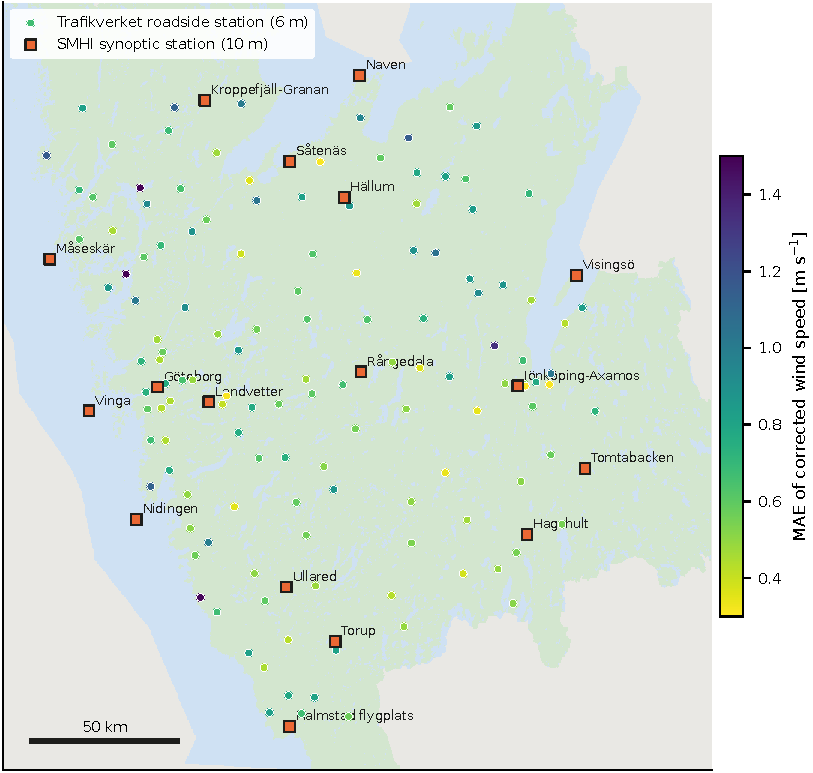
\includegraphics[width=0.85\textwidth]{figures/fig02_sweden_area.pdf}
\caption{Swedish check region: SMHI synoptic stations (squares), Trafikverket roadside stations (circles, coloured by the mean absolute error of the corrected wind speed) and road RV40.}
\label{fig:map-se}
\end{figure}

\begin{figure}[!htbp]
\centering
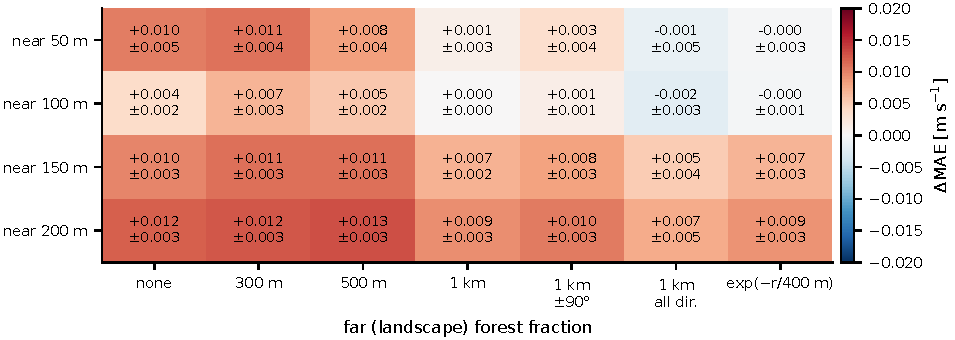
\includegraphics[width=\textwidth]{figures/fig07_two_shelter_scales_sweden.pdf}
\caption{Two shelter scales in the Swedish check region: cross-validated MAE difference ($\pm$ SE) for combinations of the near-tree radius and the landscape forest fraction, relative to \SI{100}{m} and \SI{1}{km}.}
\label{fig:twoscale}
\end{figure}

\begin{figure}[!htbp]
\centering
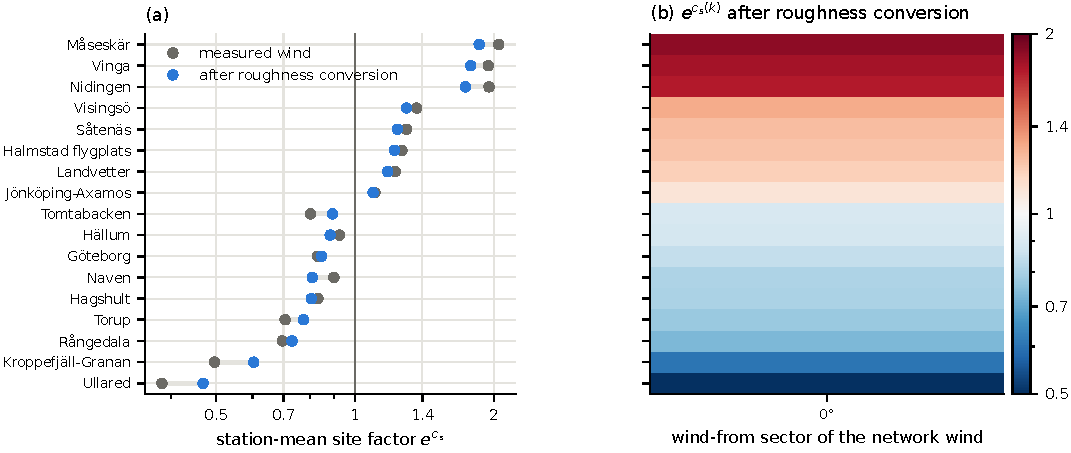
\includegraphics[width=0.8\textwidth]{figures/fig08_site_factors_sweden.pdf}
\caption{Site factors of the SMHI reference stations in the Swedish check region.}
\label{fig:site-se}
\end{figure}


\bibliographystyle{elsarticle-num-names}
\bibliography{refs}
\end{document}
